\documentclass[11pt, ngerman,english,a4]{article}
\usepackage[bottom,flushmargin,hang,multiple]{footmisc}

\usepackage[T1]{fontenc}
\usepackage{babel}
\usepackage[utf8]{inputenc}
\usepackage{xcolor} % to highlight text
\usepackage{setspace} % to doublespace
\usepackage[margin=1in]{geometry}
\usepackage[]{hyperref}
\usepackage{graphicx}
\usepackage{caption}
\usepackage{subcaption}
\usepackage{multicol}
\usepackage{amsmath}
\usepackage{color,soul}
\usepackage{bm}
\usepackage[russian]{babel}
\usepackage[sort&compress]{natbib} 
\usepackage{float}
\usepackage[labelfont=bf,textfont=md]{caption}
\usepackage{mdframed}
\usepackage{lscape}
\usepackage{ragged2e}
%\usepackage{MnSymbol}
\sethlcolor{lightgray}
\widowpenalty10000
\clubpenalty10000
\hyphenpenalty100


\setcitestyle{authoryear,open={(},close={)}}

\author{
	Lion Behrens\\University of Mannheim\\behrens@uni-mannheim.de\\
	\and
	Viktoriia Semenova\\University of Mannheim\\semenova@uni-mannheim.de
}

\date{\today }

\title{Information and Perceptions of Election Fraud, Judicial Rulings, \\ and Diffuse Political Support\vspace{0.7cm}}

 

\begin{document}
\maketitle
\thispagestyle{empty}

\onehalfspacing


\noindent \textbf{Abstract:} Consciousness of election fraud has been shown to let individuals withdraw support from candidates allegedly involved in manipulation and to depress citizens' expressed legitimacy of the elected government that stems out of processes which are perceived to be fraudulent. We outline a theory of attitudinal spillover which argues that information about electoral malpractice will lead individuals to extrapolate legitimacy loss even to political institutions that are unrelated to electoral administration. This theory predicts that consciousness about electoral misconduct will not let individuals merely detach from the institutions linked to misbehavior and the regime that surged out of an illegitimate election process, but turn their backs on the political system as a whole. Second, we examine if within-system corrections like successful court punishments of alleged fraud perpetrators can moderate decays in diffuse system support. We present the research design and analysis plan of a pre-registered online survey experiment to be conducted in Mexico and Russia as well as causal estimates from statistical matching techniques based on cross-national survey data.

\vspace{1cm}

\noindent \textbf{Keywords:} \textit{Election Fraud; Diffuse Support; Political Trust; Electoral Courts; Survey Experiment; Causal estimation.} \\ 


\vspace{2cm}

\begin{center}
  \textbf{Word Count:} 9,184.  
\end{center}



\newpage
\setcounter{page}{1}
\doublespacing

\section*{Introduction}

Which consequences do information about electoral fraud have for citizens' relationship towards their political system? Since the `electoral revolution’ that surged since the mid-twentieth century leading to a dramatic increase in the number of electoral events (\citealt{Norris2014}), competitive multiparty elections have become omnipresent across new democracies and electoral authoritarian regimes worldwide. Simultaneously, election observation has established itself as an international norm, with nearly 80\% of all federal elections in non-established democracies nowadays being monitored by international observers (\citealt{Kelley2012a}; \citealt{Hyde2011}). International monitoring missions are far from being bystanders that provide false legitimacy to flawed events through uncritical presence, as around half of all observed elections had led international missions to declare problems of moderate or high magnitude (\citealt{Kelley2012a, Kelley2012b}). At times, observation missions publicly present detailed claims of electoral misconduct and disseminate information that has the power to exert substantial influence on political affairs. Most recently, this has become evident after the 2019 election in Bolivia, where the incumbent president Evo Morales stepped down from office after serious public criticism by international monitoring groups led by the Department for Electoral Cooperation and Observation of the Organization of American States (\citealt{OAS2019}; \citealt{Idrobo2020}). 

Among the citizens themselves, credible information about electoral crimes can hold several behavioral and attitudinal consequences. Becoming conscious of electoral malpractice has been shown to lead to extreme behavior such as popular protests and violent uprisings (\citealt{Daxecker2012}). Scholars have furthermore amassed a wealth of knowledge on the effects of election fraud perceptions on individuals' attitudes towards their political authorities. First, scholars have examined how information about electoral misconduct shape individuals' evaluations of the electoral process itself.  For instance, \citet{Robertson2017} shows that providing citizens with critical reports of election observation missions considerably reduces their perceived levels of electoral integrity. Second, a branch of research has examined how election fraud perceptions relate to individuals' support of political actors. Citizens that are conscious about misbehavior withdraw support from those candidates that are allegedly involved in malpractice (\citealt{Reuter2019}) and express lower levels of legitimacy for the political regime that surged out of an electoral process that is perceived to be fraudulent (\citealt{Williamson2020}).

This article relates to theories of information processing and outlines a mechanism of attitudinal spillover which states that individuals relate specific fraud allegations to their confidence in the political system itself. The theory argues that even when information about fraud is attributed to unique political actors, citizens tend to extrapolate these to political institutions that are unrelated to electoral administration, leading to decays in levels of fundamental diffuse support for the political system as a whole. In contrast to the prior literature, the presence of such attitudinal spillovers predicts that consciousness about electoral misconduct won’t let individuals merely detach from political authorities that are directly linked to misbehavior and the regime that surged out of an illegitimate election process, but rather holds implications that are considerably more detrimental. Following the mechanism that we outline, consciousness about electoral malpractice can lead citizens to withdraw approval from the political system as a whole.

Moreover, we calibrate our theoretical predictions and outline how legal interventions from within-system actors may prevent attitudinal spillovers and moderate decays in diffuse system support (\citealt{Easton1965, Easton1975}). In a growing number of countries, individual courts play a vital role in judging the legitimacy of electoral processes, settle a number of electoral disputes, and have emerged as important actors that frequently intervene in pre- and post-electoral stages (\citealt{Eisenstadt2002}, \citealt{Kerr2020}). Especially in new democracies, courts and electoral tribunals can crucially assist processes of democratization. Public court rulings on electoral crimes may send out signals of the judiciary's professionalism, autonomy, and commitment to a fair electoral process  (\citealt{Kerr2020}). Hence, successful convictions of alleged perpetrators might therefore function as signals of at least some level of horizontal `checks and balances'. In authoritarian settings, in turn, regimes may use courts for `blame attribution' (\citealt{Beazer2019}; \citealt{Rozenas2019b}) to shift responsibilities away from regime actors themselves and towards micro-level local agents who are convicted for criminal activities in order to prevent popular disapproval of the political system they protrude. Relating these mechanisms to our theory of attitudinal spillover, we investigate whether within-system interventions as a reaction to exposed malpractice may mitigate citizens' depressed levels of diffuse support.

This paper presents the research design and pre-analysis plan of an online survey experiment to be conducted with respondents located in Mexico and Russia. In the experimental design, respondents are provided with information on a hypothetical upcoming federal election. Participants are randomly assigned to control and treatment groups and are confronted with either neutral information on electoral affairs or credible accounts of electoral misconduct. A sub-share of treated individuals is further informed about successful court convictions of alleged perpetrators of electoral misconduct. Afterwards, participants are presented a battery of questions measuring diffuse political system support incorporating a range of political institutions. We derive a variety of substantively interesting hypotheses and evaluate these using formal Bayesian hypothesis testing. Additionally, we investigate the external validity of our theory on attitudinal spillover and present causal evidence from Wave 7 of the World Values Survey (2017-2020) and 48,953 respondents across 48 countries using a variety of statistical matching techniques.  

Our article has two main contributions. First, we investigate the effect of information and perceptions of electoral misconduct on citizens’ diffuse support of the political systems as a whole. For scholars of both new democracies and autocratic politics, our study illuminates how the impact of election fraud information that is circulated after election day may have effects that are more detrimental than often thought of. In this vein, we extend previous literature that has predominantly focused on the effect of election fraud perceptions on the support for individual candidates, the direct beneficiaries of electoral malpractice, and associated behavioral consequences. This is especially interesting since diffuse support is usually seen as a stable trait that undergoes little variation in the short run. Our study sheds light on political factors that might induce it to shrink. 

Second, to the best of our knowledge, we present the very first study to investigate whether self-correcting mechanisms from within the political system can moderate and prevent withdrawal of political support as a consequence of fraud information. This holds important implications for the study of the consequences of electoral fraud across regimes. For new democracies, such effects may outline the crucial importance of horizontal `checks and balances’ for the process of democratization, as an effective justice system may play a vital role in restoring faith not only in the electoral process but the political system as a whole. In addition, our study is relevant for  scholars of electoral authoritarian regimes. If court interventions prevent dis-attachment, then regimes may be able to strategically use election tribunals and court convictions for ‘blame attribution’ (\citealt{Beazer2019}; \citealt{Rozenas2019b}), outsourcing responsibility of micro-level fraud to local actors rather than to institutional deficiencies more general.


\section*{Election Fraud Information and Diffuse Political Support}

In this section, we outline a theory of how the acquisition of new information about the integrity of domestic elections will affect the amount of trust that citizens place in the institutions of their broader political system. Essentially, this comes down to defining an argument of why individuals will extrapolate information about electoral misconduct to political institutions that are unrelated to electoral administration. 

\subsection*{Election Fraud Information and Attitude Extrapolation}

Scholarly contributions that examine the attitudinal nexus between citizens and the state commonly refer to David Easton's (1965, 1975) work on ‘system support’ as a joint conceptual heritage. The theoretical distinction that is most relevant for our argument is the classical discrimination between diffuse and specific levels of support. Specific support refers to the relationship between members of a system and the specific actions and decisions of political authorities that reside within its institutions. As such, specific support relates to the evaluations of the day-to-day actions of political leaders, and are highest if perceived outputs match citizens’ articulated demands (\citealt{Easton1975}, p. 438). In contrast, diffuse support describes individuals’ generalized attachment to the political system. According to Easton, \textit{"[diffuse support] refers to evaluations of what an object is or represents [..] not of what it does. [..] Whereas specific support is extended only to the incumbent authorities, diffuse support is directed towards offices themselves as well as their individual occupants. More than that, diffuse support is support that underlies the regime as a whole and the political community."} (\citealt{Easton1975}, pp. 444-445). Hence, diffuse support is \textit{a priori} expected to be more durable than citizens’ performance evaluation of specific political authorities. While positive evaluations of actors’ performance is volatile and comes with consistent rise and fall, diffuse political support for the entity of the political system is in general thought to be long-lasting. 

Early work on the concept of political support did almost exclusively focus on the relation between citizens and the state in the context of the United States and other advanced industrialized democracies (\citealt{Easton1965, Easton1975}; \citealt{Citrin1974}). Importantly, already in their seminal work on popular support for authoritarian regimes, \citet{Geddes1989} have argued that political reasoning in democracies and autocracies can be expected to operate in similar ways and a range of studies have evaluated concepts derived from the distinction of specific and diffuse support in autocratic settings as well (\citealt{Reuter2019}; \citealt{Frye2019}). In addition, it has been shown that measurement equivalence of the most prominent operationalizations of diffuse support holds and can be analyzed across a variety of regime types (\citealt{Schneider2017}). 

In the first place, we can expect that credible fraud information evolving around electoral contests will lower citizens’ confidence in such. For instance, both \citet{Robertson2017} as well as \citet{Bush2018} show that confronting voters with criticisms from election observer groups reduces their evaluations of electoral quality and the legitimacy of the electoral process. In the literature evolving around system support, it has long been argued that attitudes about the performance of individual objects that are commonly associated with specific support can spill over to more generalized attachments towards the political system (\citealt{Bowler2004}). This goes contrary to an assumption that citizens’ evaluations of \textit{political actors} are unrelated to their evaluation of their \textit{political institutions}. Empirically, spillover-like effects are a well-established phenomenon in various branches of attitudinal research. In general, these can be understood as specific manifestations of a more general psychological principle commonly referred to as the `halo effect’ by which individuals ascribe characteristics to a person or an object based on their evaluation of other empirically observable object-related characteristics even if the individual traits are unrelated to each other (\citealt{Thorndike1920}; \citealt{Palmer2016}). Such spurious inferences may result from individuals’ inability to differentiate between different characteristics and may even occur if there is sufficient information to allow for independent assessments in the first place (\citealt{Nisbett1977}). Regarding citizens’ evaluations of actors and institutions, it has been shown that trust in national institutions transcends to trust that is placed in the international arena, extrapolating federal-level experiences to European institutions (\citealt{Torcal2019}) and international organizations (\citealt{Dellmuth2015}). Studying attitudinal spillovers between national institutions, \citet{Bowler2004} show that political scandals of individual politicians have the power to erode confidence in executive institutions and the government in general. 

Notably, such spillover effects may either be the result of evaluating a series of repeated outputs over a long time series that can change even fundamental beliefs, or chief, salient, and decisive short-term experiences that transform into fundamental attitudes more rapidly. We hypothesize that information about electoral fraud provide the kinds of short-term information that dis-attaches from the volatile performance of political actors and transforms into generalized evaluations even of other components of the political system. 

Essentially, this is based on a two-step argumentation line. First, as elections lie at the core of democratic accountability and are the one crucial element common to all and even minimalist definitions of democracy (\citealt{przeworski_stokes_manin_1999}), systematic misbehavior that evolves around the decisive process of elections is likely to be taken as informative not only of what a specific political object does, but even towards the system that it represents. Hence, the central place of well-conducted elections in the constitution of a democratic political system lets evaluations of the electoral process fundamentally differ in their nature from perceived output that is generated through the short-term and volatile performance of individual office holders. This provides election-related information with the general \textit{possibility} for producing spillovers. Second, it has been shown by a variety of authors that citizens tend to fail in \textit{distinguishing} their attitudes towards individual components of the multidimensional political system. This is most evident as the political sphere is usually described to be too complex to understand even for highly informed individuals (\citealt{zaller_1992}) and as citizens need lower-complexity informational cues to maneuver their perceptions of political affairs. Empirically, scholars have long found that support levels for different political institutions or entities are highly correlated with each other and are often hard to disentangle within individual respondents (\citealt{Hooghe2012}; \citealt{Mishler2001}). It is these two observations that build the premises from which motivate the central claim of this paper. (i) The  centrality of election-related information for citizens’ evaluation of the political system which provide the possibility for spillover fused with (ii) the general tendency of individuals to fail distinguishing support for different institutions lead us to formulating our main hypothesis: \\
	
\indent \textit{Hypothesis 1: Individuals who are exposed to information about electoral fraud show less confi- \indent dence in other institutions of the political system that are unrelated to electoral administration.} \\

It is worth noting that while our hypothesis relates to mean differences between the distributions of individual support rates, there are two plausible mechanisms of how this mean shift may come to rise with regard to pre-existing individual characteristics. Arguments related to motivated reasoning suggest that individuals show a tendency to specifically sort out those informational cues that affirm their prior beliefs for opinion formation and ignore cues that contradict them (\citealt{Robertson2017}, \citealt{Bush2018}). This may lead individuals to selectively respond to information that matches their prior belief. In the political sphere, partisanship is key. Regarding attitudinal spillovers, \textit{regime opponents} may be those that particularly respond to fraud information since it further strengthens their pre-existing political beliefs which extrapolate to diffuse support levels. Regime supporters, in contrast, might simply discard election fraud information as dissonant to their world view and attribute it to mere opposition strategies. In this line of reasoning, we should see spillover effects among regime opponents but not among supporters. 

On the contrary, theories that might be labeled as a logic of Bayesian belief updating have prominently been put forward in the information processing literature (\citealt{Bullock2009}; \citealt{Hill2017}). \citet{Reuter2019} show that when revealing information about systematic interference, especially \textit{regime supporters} withdraw support from regime candidates that allegedly engaged in fraud as it these respondents for which the information actually makes a difference and can change their ex ante beliefs that elections are actually free and fair. While providing regime supporters with information on election fraud provides them with an opportunity for a change in beliefs, regime opponents already believe in fraudulent elections ex ante and might be unaffected by new information. In this line of reasoning, the spillover effect might be particularly strong among regime supporters. While we deem it important to closely trace which of these mechanism ultimately leads to our hypothesized mean difference between distributions of diffuse support levels, we note that both are in line with the central claim as formulated in Hypothesis 1. 


\subsection*{Previous Literature}
While examining the empirical interrelations between operationalizations of specific and diffuse support is a decade-old endeavor, the attempt to link system support with election fraud information is rather new. Our specific research strategy tabs into a broader field of previous studies that have examined related phenomena which are relevant for our expectation. A branch of studies focused on the relation between `objective’ measures of electoral manipulation and average levels of diffuse support. \citet{Mauk2019} globally assembles expert-coded judgements of federal-level electoral integrity from the Varieties of Democracy dataset and relates these to national levels of political trust, finding little evidence that objectively coded factual levels of electoral integrity are related to country-specific average values of political trust. Exploiting largely exogenous variation in a survey conducted in Moscow around the 2011 Russian \textit{Duma} elections, \citet{Frye2019} reach similar conclusions and find that simply the mere event of an allegedly fraudulent election does not significantly reduce levels of diffuse support when comparing those individuals that have been surveyed after the election with the respondents whose data has been collected beforehand. These studies carry the obvious shortcoming that they calculate effects of \textit{a posteriori} collected fraud indicators on all individuals that might potentially have become aware of such information. However, as \citet{Mauk2019} outlines, actual electoral malpractice does not necessarily need to be related closely to citizens’ individual perceptions of electoral integrity (see also \citealt{VanHam2015}), since these crucially depend on factors such as a sufficiently free media environment to report about electoral inferences and one's individual political interest to become informed through media channels. 

A different group of authors directly exposes individuals to information about electoral malpractice and investigates how becoming aware of misbehavior affects citizens’ beliefs about the electoral process (\citealt{Robertson2017};  \citealt{Bush2018}) and their support for candidates that are allegedly involved in malpractice (\citealt{Reuter2019}). These studies shed great light into individuals opinion-formation dynamics as a response to sensitive information, but restrict their analyses to attitudes that are directly linked to the electoral process or to specific evaluations of office holders rather than examining underlying attachments towards the political system.    

Using World Values Survey data, \citet{Norris2014, Norris2019} exploits a cross-sectional design and shows that even when controlling for a range of attitudinal and socio-demographic factors, expert evaluations and perceptions of electoral integrity are still correlated to an array of items as wide as confidence in elected institutions such as parliaments and governments, overall satisfaction with performance of democracy and respect for human rights. Obviously, using such cross-sectional strategies, it as hard to disentangle whether perceptions of electoral integrity and institutional confidence are simply observed jointly, or if one determines the other, falling short in testing a spillover theory as outlined here.  Even if a directional effect exists, the flow of causality might well flow into the opposite direction. It is not less reasonable to assume that stable underlying beliefs such as confidence in political authorities pre-structure individuals’ evaluations of specific political events such as electoral contests. 

In the piece that is most relevant for our research, \citet{Williamson2020} shows how confronting citizens with condemnations of international election monitors can reduce expressed legitimacy in the political regime that surged out of an allegedly fraudulent process. Using correlational analysis from eight Arab countries and a survey experiment conducted in authoritarian Egypt and Morocco, he shows how perceptions of electoral misconduct hinder both attitudinal and behavioral compliance with a regime’s rule. This investigation of individual conformity with the direct beneficiary of misbehavior is considerably different from our spillover perspective which investigates effects even towards components of the multidimensional political system that are unrelated to fraud information as coined by the Easton’s concept of diffuse support. 

%In sum, each one of these studies enhances our understanding of the nexus between electoral integrity and citizens’ attitudes by employing cross-sectional designs, operationalizing election fraud through objective measures of electoral integrity, or studying the effect of election fraud information on attitudes towards individual political actors and the regime that surged out of an allegedly fraudulent process. In this contribution, we are interested in the direct causal effect of election fraud information itself and focus on citizens’ fundamental attachments to the political system as a whole rather than on evaluations of individual political actors or merely the electoral process. 

\section*{Electoral Crimes and Court Rulings}
In this second part of our theoretical scrutiny, we calibrate our theoretical expectation and outline how spillover effects might be changed if third-party system actors become active as a consequence to fraud allegations. How does the spillover effect of election fraud information behave against credible interventions from within the political system? In recent decades, courts have played an increasingly important role in electoral politics. Courts have emerged as an important actor that settles electoral disputes and frequently intervenes in pre- and post-electoral stages when the electoral conduct is in doubt (Eisenstadt 2002; Kerr and Wahman 2021). The topics that are covered by electoral tribunals range from issues revolving around constructing valid and comprehensive voter registers, the confirmation of candidate or party lists and the regulation of campaign resources up to sensitive issues such as election day fraud and vote manipulation. Court rulings on electoral crimes are highly salient for the electorate as they provide citizen with key non-partisan political information which regularly makes headlines in federal newspapers. %(\hl{cite cases}).

A substantial branch of literature has outlined that citizens’ perceptions of electoral fairness is dependent on the actions of the judicial branch (\citealt{Kerr2020}). It is important to note that (the absence of) court interventions can play vital roles for the \textit{spillover} effect from exposure to electoral misconduct towards attitudes related to the political system. Specifically, we can expect court rulings to directly affect the dynamics of attitude extrapolation. We focus on two specific arguments: the \textit{amplifying spillover} and the \textit{spillover prevention} argument. 

The amplifying spillover argument is rooted in the empirical observation that electoral quality is so routinely disputed in new democracies and authoritarian regimes that without third-party actor activities, opposition parties’ or losers’ protests may simply be perceived as a conventional ‘part of the game’ (\citealt{Kerr2020}). From this perspective, defeated candidates are incentivized to publicly condemn the electoral process in order to avoid seeming weak in front of their voter base and to discredit the authority of the political opponent (\citealt{Lindberg2006}). The potential spillover effects from acquiring information about electoral misconduct may hence in general be depressed by voters’ doubts whether the allegation itself is credible. 

When alleged perpetrators of electoral crimes are sentenced in front of the judiciary, the presence of court convictions in turn provide an official recognition that the election process was not free and fair and send credible signals about the trustworthiness of fraud claims. Under this logic, court rulings provide the public with detailed information about the nature and scope of electoral malpractice and may serve as a heuristic device for voters to reliably evaluate electoral fairness based on the statement of third-party actors. As such, court convictions can be expected to lead to a stronger spillover effect, as courts confirm the deficiencies in the political system as suggested by information on the presence of electoral manipulation. \\

\indent \textit{Hypothesis 2a: The attitudinal spillover effect of election fraud information is stronger for indi- \indent viduals who are exposed to information about successful court convictions of alleged perpetrators \indent for electoral crimes.} \\

The line of reasoning emphasizing the spillover prevention potential of court rulings builds on the idea that independent interventions of the justice system into the electoral process might signal information about the quality of the political system as a whole. Court rulings may be interpreted as a sign of autonomy and professionalism that goes in counter to information about electoral fraud that signals system deficiencies. Convictions in front of electoral tribunals may lead to individual perceptions that the system of checks and balances in the country works reasonably well and that the political system does indeed have the capacity for self-correction if elections fail to meet shared standards.  In this line of argumentation, court rulings show that it’s not the political system \textit{as a whole} that is foul, but that state institutions do have the capacity to offer counterweights to the malpractice of other institutions. As a consequence, interventions of courts may reduce the spillover to decays in diffuse support for other political institutions. An additional argumentation line for the spillover prevention effect can be derived from scholarly contributions on  authoritarian politics. In electoral authoritarian regimes, it has been outlined how political authorities may use political events for `blame attribution’ in which positive news is selectively attributed to the regime and the responsibility for bad news is blamed on external factors (\citealt{Beazer2019}; \citealt{Rozenas2019b}). Similarly, political actors can use court convictions to outsource the responsibility for electoral malpractice to micro-level agents and deny their interrelation with the political system in front of the citizenry. This leads us to formulate a contrasting expectation to Hypothesis 2a, namely: \\

\indent \textit{Hypothesis 2b: The attitudinal spillover effect of election fraud information is weaker for indi- \indent viduals who are exposed to information about successful court convictions of alleged perpetrators \indent for electoral crimes.}

\section*{Research Design}

\subsection*{Case Selection}

We test these arguments on (i) the attitudinal spillover of election fraud perceptions towards institutions that are unrelated to electoral administration and (ii) the moderating role of electoral rulings using data from a pre-registered online survey experiment to be conducted with respondents located in Mexico and Russia in 2021.\footnote{This document lines out the case selection, research design and identification strategy underlying our survey experiment. Data collection itself will be conducted between February and March 2021.}\footnote{We will pre-register the setup of our survey experiment and the concrete steps in our statistical analysis.} The main advantage of focusing on these two countries is that they share a variety of features which are relevant for our experimental design. In both cases, we study middle-income countries whose party systems have shown a relatively high level of stability throughout past decades and who share a large history of public controversies around electoral fraud. 

In the post-World War II era, Mexico underwent a gradual and often described as pendular democratization process (\citealt{Cantu2015}; \citealt{Hiskey2005}). Although since the end of the Mexican Revolution, elections were held regularly in six-year intervals and political opposition was granted passive voting rights, the authoritarian rule of the Institutional Revolutionary Party (PRI) effectively consolidated a hegemonic one-party party system (\citealt{Sartori1976}) with only few local opposition parties far from national influence existing parallel to the official administration. Popular distrust in the legitimacy of Mexican elections roots in the experience of PRI’s one-party rule which was notoriously engaged in attempts of electoral manipulation against both sides of the political spectrum. PRI’s strategies in balancing out authoritarianism with competitive elections manifested in unrecognized victories of the right-wing PAN party in a multitude of subnational elections in the 1980s and 1990s (\citealt{Greene2007}; \citealt{Cantu2015}), systematic repression against the left-winged Democratic Revolution Party’s (PRD) candidates (\citealt{Greene2007}), and election-day fraud such as the manual alteration of vote tallies in a series of regional and national-level contests (c.f. \citealt{Cantu2019b}).

It was not before the 1980s that electoral competition led to more inclusive electoral contests which produced changing majorities. First, recognized opposition victories occurred in state-level and local elections and only recently culminated in the first national-level contest since the Mexican Revolution of 1920 being decided in favor of the political challenger when the National National Action Party’s (PAN) candidate defeated PRI’s Francisco Labastida in July 2000. Today, Mexico’s political party system shows a remarkable level of institutionalization when compared to other new democracies and locates the country on the upper end of the scale of party system stability in Latin America (\citealt{Greene2018}). Notably, the historical baggage of electoral maladministration and attempts of manipulation persists and reaches forward up until the country’s most recent electoral events (\citealt{Cantu2014}; \citealt{Cantu2019a}). 

In Russia, we study a context of institutionalized authoritarian rule. After the dissolution of the Soviet Union in 1991, meaningful opposition has effectively been banned since the beginning of Vladimir Putin’s administration in 1999 and several observers note that election-day fraud has metasized since in the earlier 2000s (\citealt{Myagkov2009}). Today, Russian federal elections are frequently accompanied by widespread protests for instance after the Russian Duma elections of 2011 in which considerable protests of up to about 150,000 participants were witnessed in Moscow, St. Petersburg and regional capitals (\citealt{Robertson2017}). Electoral monitors routinely condemn Russian elections and a whole range of scholarly contributions focuses on highly unusual patterns in published voting returns that are hard to explain with processes that exclude the manual alteration of vote counts (\citealt{Rozenas2017}; \citealt{Klimek2012}; \citealt{Myagkov2009}; \citealt{Jimenez2017}; \citealt{Kobak2016a, Kobak2016b, Kobak2018}). Experimental evidence suggests that in the 2011 parliamentary vote, the vote share of the incumbent United Russia party was at least 11 percentage points lower than documented by official figures (\citet{Enikolopov2013}). Nowadays, only about 15.5\% of Mexicans and about 39.8\% of Russians say that election officials are fair and that votes are counted free and fairly.\footnote{Source: World Values Survey Wave 7 (\citealt{Inglehart2020}), 2017-2021.}

%Moreover, Mexico and Russia serve as excellent cases in which to examine the moderating effect of court interventions on attitudinal spillovers stemming from electoral fraud perceptions since both countries are characterized by active courts that have publicly convicted people of electoral crimes. \hl{Outline how courts play a role and have convicted people. Describe how they evolved in Mexico and Russia, maybe give 1-2 examples of rulings. In Mexico, developed as independent actors. In Russia, dependent on executive power, filled with loyalists appointed by governments, strong ties between judiciaries and incumbent parties.} 


\subsection*{Survey Design}
The survey itself is set up via the online platform \textit{SoSci Survey} and distributed to respondents using the platforms \textit{Amazon Mechanical Turk} in Mexico and \textit{Yandex} in Russia. The survey takes about ten minutes to complete and starts off with a range of socio-demographic identifiers and several questions on political attitudes that are relevant to our expectations. Subsequently, respondents are assigned to treatment and control groups.\footnote{See the Appendix for a preliminary version of the survey questionnaire.} We aim at a sample sizes of about $n=500$ respondents in each country. A considerable number of studies have evaluated the use of crowdsourcing marketplaces for social science research (\citealt{Bartneck2015}; \citealt{Berinsky2012}). An obvious shortcoming of our data collection is that not all societal groups are equally well represented on the platforms that we use for the acquisition of participants. Based on previous studies investigating demographic predictors of participation in manual crowdsourced labor, we can confidently assume that our survey is predominantly conducted among urban internet users who are younger than the general population and obtain some level of higher education (\citealt{Berinsky2012}). 

Regarding respondents in Russia, recent surveys on educated, urban, internet-using citizens have shown that even among these demographic strata, which are often thought to hold views that are particularly opposed to the regime, attitudes towards incumbents and political authorities are very much divided. This makes us confident that we will cover both regime supporters and opponents in our online data collection (\citealt{Robertson2017}). Additionally, the sampling strategy that we adopt here provides some concrete advantages over nationally representative surveys. First, the demographic groups that we are likely to sample show higher awareness of election monitoring groups (\citealt{Robertson2017}). This assures that respondents give valid answers and, through their background knowledge, can accurately assess the meaning and implications of our treatments. Second, the socio-demographic profile of our survey respondents specifically targets those population groups that are particularly important for political dynamics such as gathering and sharing sensitive regime information and boosting their publicity by carrying them to the streets in protests. Both in Mexico (\citealt{Inclan2017}) and in Russia (\citealt{Rosenfeld2017}), studies have shown that the population groups that we survey using online crowdsourcing platforms are those that are particularly prone to participate in political protests.  

In addition, it is worth noting that while the specific attitudes of these surveyed groups might not be representative of the population as a whole, there is a wealth of evidence amassing that the factors which shape these attitudes are. Research has shown that treatment effects within attitudinal research based on data collected using \textit{Amazon MTurk} are similar to those found in representative surveys (\citealt{Clifford2015}; \citealt{Coppock2019}).\footnote{Similar conclusions have been reached independently from each other across a variety of disciplines (\citealt{Bartneck2015}; \citealt{Yang2015}).} Hence, while our sampled group differs from the general population in terms of their attitudes descriptively, we might well expect the general patterns around their reactions to the experimental stimuli that we formulate our hypotheses on to hold in the general population. 

\newpage

\subsection*{Causal Identification}

The experimental design is centered around levels of diffuse support towards the political system and exposes respondents to one of three experimental groups. After answering the introductory questions of the survey, respondents are randomly assigned to one of the text fragments described in Table \ref{tab:treatments}. The text of the first group is neutral and states some basic facts about a hypothetically upcoming federal election to elect the country’s main legislative body. The second text contains the general information about the election scenario, but additionally exposes respondents to information about malpractices that were allegedly performed on election day. It details accusations of a group of domestic and international observation missions and follows experimental set ups such as those to be found in \citet{Bush2018}, \citet{Williamson2020} and \citet{Robertson2017}) who also used evaluations of election observer missions as credible measures for fraud information. The information presented to the third group goes beyond the presentation of general facts about the hypothetical election as well as the description of fraud allegations and exposes respondents to information about punishments from within the political system directed at those individuals who are allegedly responsible for electoral crimes. The punishment includes legal actions in which alleged perpetrators were legally convicted for the performance of electoral crimes and personal consequences within electoral commissions that alleged perpetrators have worked for. In order to ensure that exactly one third of all respondents per country are placed in in each of the three experimental groups and to avoid sparse data problems that might arise from extreme scenarios under complete randomization, we apply a randomized block design separately for each of the country cases under scrutiny. 

After being confronted with these information, respondents are presented a battery of questions measuring their levels of diffuse support for individual institutions of their political system. The most prominent empirical conceptualization of \citet{Easton1975}'s classical concept of diffuse support  is political trust (\citealt{Hooghe2012}; \citealt{Schneider2017}; \citealt{Frye2019}). Specifically, we ask each participant the following question: \textit{“Upon receiving this information, how much confidence would you have in the following organizations or institutions?”}. The battery of items includes \textit{“(1) the armed forces, (2) the police, (3) the press, (4) the justice system/courts, (5) the government, (6) the parliament and (7) political parties"}. Responses are collected on a seven-point scale ranging from “none at all” to “a lot” as standardly employed in cross-national survey programs. 

\singlespacing
\begin{table}[H]
    \caption{Experimental Treatments.}
    \label{tab:treatments}

\hrule \\
\vspace{0.5cm}
\textbf{(1) Control group: Neutral information} \\
Suppose that federal legislative elections for the \textit{[Champer of Deputies/State Duma]} were held in \textit{[month]} of this year. Imagine that as usual, also in this hypothetical election more than 2,000 candidates competed for the \textit{[500/450]} parliamentary seats. Suppose that all parties that are currently presented in the \textit{[Champer of Deputies/State Duma]} have retained positions in the assembly and that the incumbent party \textit{[MORENA/United Russia]} has won the largest seat share. \\

\textbf{(2) Treatment group: Fraud information} \\
\hl{$[$Neutral information$]$} \\
On an after election day, however, allegations of ballot-box stuffing and alterations of vote tallies perpetrated by individuals working for electoral commissions in favor of the incumbent party were widespread. Shortly after election day, a number of domestic and international election observation missions publicly called out a variety of electoral misconducts and manipulation practices across several regions of the country. \\

%\textbf{(3) Treatment group: Fraud information with electoral commission punishment} \\ 
%\hl{$[$Neutral information$]$} \\
%\hl{$[$Fraud information$]$} \\
%As a consequence, \textit{[the Federal Electoral Institute INE/superior electoral commissions]} took action and individuals allegedly responsible for fraud lost their positions in electoral commissions. \\

\textbf{(3) Treatment group: Fraud information with court punishment} \\
\hl{$[$Neutral information$]$} \\
\hl{$[$Fraud information$]$} \\
As a consequence, legal action was brought against individuals allegedly responsible for fraud which were convicted for electoral crimes by responsible courts and lost their position in electoral commissions.
\vspace{0.5cm}
\hrule
\end{table}
\doublespacing

A range of important characteristics of the experimental design can be noted in relation to the spillover theory that was outlined in previous sections of this manuscript. First, the text fragments that are presented to members of the treatment groups explicitly discuss the \textit{mechanisms} of alleged election day fraud. This is because we want to avoid the presence of heterogeneous effects as a consequence of vague fraud information which calls different interpretations of our fraud treatment, for instance associations of vote buying in Mexico (\citealt{Cantu2019a}) and ballot box stuffing in Russia (\citealt{Myagkov2009}). Second, referring to `individuals working for electoral commissions’, we explicitly state the alleged \textit{perpetrator of fraud}. Mentioning the perpetrator is crucial as it allows us to directly study if trust is extrapolated to different bodies that are unrelated to administration of elections. 

Note that not all of the institutions that we include in our battery on political trust allow us to unambiguously identify spillover effects. For example, it is hard to disentangle whether fraud in new democracies or electoral authoritarian regimes constitutes the actions of micro-level agents or whether these practices are instructed from party representatives. For citizens who expect the latter, information about election day fraud may actually function as informational cues implying partisan involvement from political authorities. Among these participants, changes in diffuse support for the three latter institutions (5)-(7) of the government, parliament and political parties may not necessarily be the result of an attitudinal spillover following from trust extrapolation as we theorize, but a straightforward withdrawal of political support from the perceived perpetrator of electoral misconduct. While substantively relevant, this scenario would not provide evidence for our outlined theory on information processing, which focuses on the \textit{extrapolation} of trust which spills over to unaffected branches of the political system.

We undergo two strategies to counter this possibility. First, we ask for respondents’ levels of disuse support towards a variety of institutions (1)-(4) that are clearly exogenous to our fraud treatment. Without spillover, trust in institutions such as the armed forces, the police, the press or the justice system are unaffected by information on election day manipulation, as members of these institutions are unrelated to fraudulent interference practiced by individuals working for electoral commissions on voting day. In contrast, decays in diffuse support towards these institutions as a response to our fraud treatments present genuine spillover effects. Second, in order to disentangle whether changes in diffuse support for the institutions (5)-(7) of the government, parliament and political parties represent genuine spillover effects as stated by Hypothesis 1 or merely a direct withdrawal of support from assumed perpetrators, we include a follow-up question after our treatment and the responses to the political trust battery asking: \textit{“Some people say that there are systematic irregularities to be observed in the federal elections of [country], while other people deny that. Given that such claims were true, to which extent do you expect representatives of political parties and state-affiliated agents to be involved?”}. Changes in diffuse support among those respondents who do not expect party representatives playing a role in fraudulent interference are considerably less prone to treatment endogeneity and hence provide a more realistic estimate of the causal effect even towards institutions (5)-(7) that might be implicitly associated with our fraud treatment. 

\section*{Analysis and Findings}

\subsection*{Statistical Modeling}

To test Hypothesis 1, we are interested in the mean difference between the control group (1) and those individuals that are assigned to treatment group (2) in Table 1. To evaluate Hypotheses 2a and 2b, we specifically contrast mean differences between groups (1) and (2) with the mean differences between groups (1) and (3). 

Although the random assignment of respondents to treatment and the control groups allows for an unbiased estimate of our treatment effect, we present additional models alongside the raw effects and present adjusted mean differences which take into account a range of socio-demographic information which might influence responses to the outlined fraud treatments and political attitudes such as levels of diffuse support. Since research has provided consistent evidence that perceptions of electoral fairness are divided by partisan lines (c.f. \citealt{Cantu2015}), we include two measures of political support. We ask individuals to which extent they support the current incumbent government and request them to report their partisan identification. Since younger, urban and highly educated individuals have been found to show the highest protest propensities in new democracies and electoral authoritarian regimes, we include measures of age, urbanity and the \textit{ISCED-2011} scale as a measure for education in our models. As we know that individuals’ levels of social and political trust are related and individuals’ `generalized trust in the world’ might well predict their responses to our fraud treatments and their levels of diffuse support, we include a measure of interpersonal trust asking \textit{“Generally speaking, would you say that most people can be trusted or that you need to be very careful in dealing with people?”}. Since private sector workers and individuals employed by the state itself may hold different views towards the political system, we include a dummy indicating private sector workers. Additional controls include measurements for gender, occupational status, household income and individuals’ position on the left-right scale.  

Since our dependent variables take on the form of ordered categorical vectors comprising seven categories $j$ ($j=1,...,7$), we calculate a set of ordered logistic regressions which can be formalized as

\begin{equation}
 \begin{split}
log(\frac{p(y^{m}_i \leq j)}{p(y^{m}_i > j)}) & = \alpha_j - (\theta_1 T_i^{fraud} + \theta_2 T_i^{punish})  \\
log(\frac{p(y^{m}_i \leq j)}{p(y^{m}_i > j)}) & = \alpha_j - (\theta_1 T_i^{fraud} + \theta_2 T_i^{punish} + \bm{\beta} \bm{X}) 
\end{split}
\end{equation}

\noindent where $y^m_i$ is the level of diffuse support of an individual $i$ ($i=1,...,n$) for one particular institution $m$ ($m=1,...,7$), $T_i^{fraud}$ and $T_i^{punish}$ are binary variables denoting membership in the experimental groups (2) and (3)\footnote{Individuals in the control unit serve as the reference category in our analysis.}, $\bm{X}$ is an $i \times k$ vector of covariates ($k=1,...,k$), $\alpha_j$ are threshold parameters, $\bm{\beta}$ are the regression parameters for the covariates and $\theta_1, \theta_2$ are the main parameters of interest.

For parameter estimation, we employ a fully Bayesian framework for statistical inference as implemented in Stan (\citealt{StanDevelopmentTeam2020}). Specifically, we rely on Hamiltonian Monte Carlo sampling in which priors are defined to follow Gaussian distributions, are centered around zero and take on a sufficiently large variance to ensure that priors are uninformative and do not favor any of the substantial hypotheses. We run a set of two Markov chains out of which we discard the first 10,000 as warm-up and use the following 50,000 samples to describe posterior distributions. We check for model convergence using the Gelman-Rubin diagnostic and consider models converged if the discrepancy measure stays below 1.1 (\citealt{Gelman2004}).

While relying on a Bayesian framework holds general advantages as it allows us to state the uncertainties around our results in straightforward probabilistic statements, it provides very specific advantages to our substantive questions at hand. As our hypotheses on the moderating effect of court rulings evolve around two competing expectations expressed in Hypothesis 2a and 2b, we exploit formal Bayesian hypothesis testing using the Bayes factor defined as 

\begin{equation}
    BF_{ab} = \frac{m(H_{2a}|y,\bm{X})}{m(H_{2b}|y,\bm{X})}
\end{equation}

\noindent to comparatively quantify to which extent the data favors one hypothesis over the other (\citealt{Kass1995}; \citealt{Gill2015}). For Bayes factor estimation, we rely on the approximate adjusted fractional Bayes factor as developed by \citet{Gu2018} and implemented in the package \texttt{bain} (\citealt{bain2020}) within the R software environment (\citealt{R2020}) that is particularly well suited for the evaluation of competing directional hypotheses. 

\subsection*{Empirical Results}

\vspace{1cm}

\begin{center}
    [RESULTS OF OUR SURVEY EXPERIMENT HERE]
\end{center}

\vspace{1cm}

\section*{Cross-Country Evidence}
We now trace further empirical implications of our theory on a broader sample. Specifically, we test whether the proposed mechanism is in line with evidence from survey data from a heterogeneous country setting using statistical matching techniques for causal inference. To evaluate our central hypothesis of attitudinal spillover, we investigate whether effects of election fraud perceptions on diffuse support for political institutions that are unrelated to electoral administration also hold in a larger sample and a more heterogeneous country setting. To this end, we leverage data from the World Values Survey, a large-scale cross-national survey program relying on nationally representative samples providing time-series data between 1981-2020. 

While survey items relating to Easton’s (1965, 1975) concept of diffuse support are part of the core questionnaire and asked consistently throughout all waves, a comprehensive battery of questions assessing respondent’s perceptions of their country’s electoral integrity has not been introduced before Wave 6 (2010-2014, c.f. \citealt{Norris2014}). Because perceptions of electoral fraud are not randomly assigned among respondents, individuals may differ from each other in ways that are related to their fraud perception as well as their diffuse support for political institutions. The World Values Survey includes a rich set of covariates that make it possible to condition on possible differences between individuals. 

After screening the data files, we noted that in particular Wave 7 (2017-2020) of the cumulative data file provides questions on issues that are particularly relevant for potential confounding mechanism that we are confronted with in the study of fraud perceptions and diffuse support. In particular, one can imagine that attitudes towards broader issues such as political corruption \textit{in general} may locate individuals on scales measuring perceptions of practices of election day fraud and confidence in political institutions. Moreover, citizens’ levels of \textit{generalized trust} in the world may condition perceptions of election day events and the particularities of a political system (c.f. Keele 2007). The covariates that we employ are `pre-treatment’ in the sense that they either portray socio-demographic characteristics that are unaffected by respondents’ evaluations of election day practices or report more generalized attitudes that are likely to be preceding in the causal chain when explaining `treatment’ variation of fraud perceptions.\footnote{One issue with our procedure is that the attitudinal measures are not strictly preceding the main variables of interest and might thus be \textit{affected} by fraud perceptions and confidence in institutions rather than \textit{predicting} `treatment' status. We report estimates including the attitudinal measures, but note that the results are robust to model specifications which only use socio-demographic information for covariate adjustment.} We hence exploit data from Wave 7 of the World Value Survey covering 48 different countries across democratic and electoral authoritarian regimes. Table A1 in the appendix provides an overview over our used variables and countries included in the analysis. Our final models include a total number of 48,953 respondents. 

Regarding our measures of fraud perceptions and diffuse political support, we choose those variables that provide the closest approximation of the measurements imposed in our survey experiment to ensure a direct test of external validity. The World Values Survey measures diffuse support through asking respondents: \textit{“I am going to name a number of organizations. For each one, could you tell me how much confidence you have in them: is it a great deal of confidence, quite a lot of confidence, not very much confidence or none at all?”}. We include responses to the same seven institutions that we collect data on in our survey experiment. On the explanatory side, rather than assigning participants to different kinds of fraud information, respondents here are asked about a battery of items covering various aspects of electoral integrity throughout the whole electoral cycle. We focus on the question that is most closely related to the mechanism of election day ballot fraud of our survey experiment stating: \textit{“In your view, how often do the following things occur in this country’s election: Votes are counted fairly.”}. Answers are collected on a four-point scale covering “very often”, “fairly often”, “not often” and “not at all often”. To straightforwardly discriminate `treatment’ and `control’ groups, we collapse this variable into a binary indicator with each group covering two response categories.  

\begin{figure}[H]
    \caption{Covariate Balance Before and After Sample Adjustment Using Coarsened Exact Matching.}
    \centering
    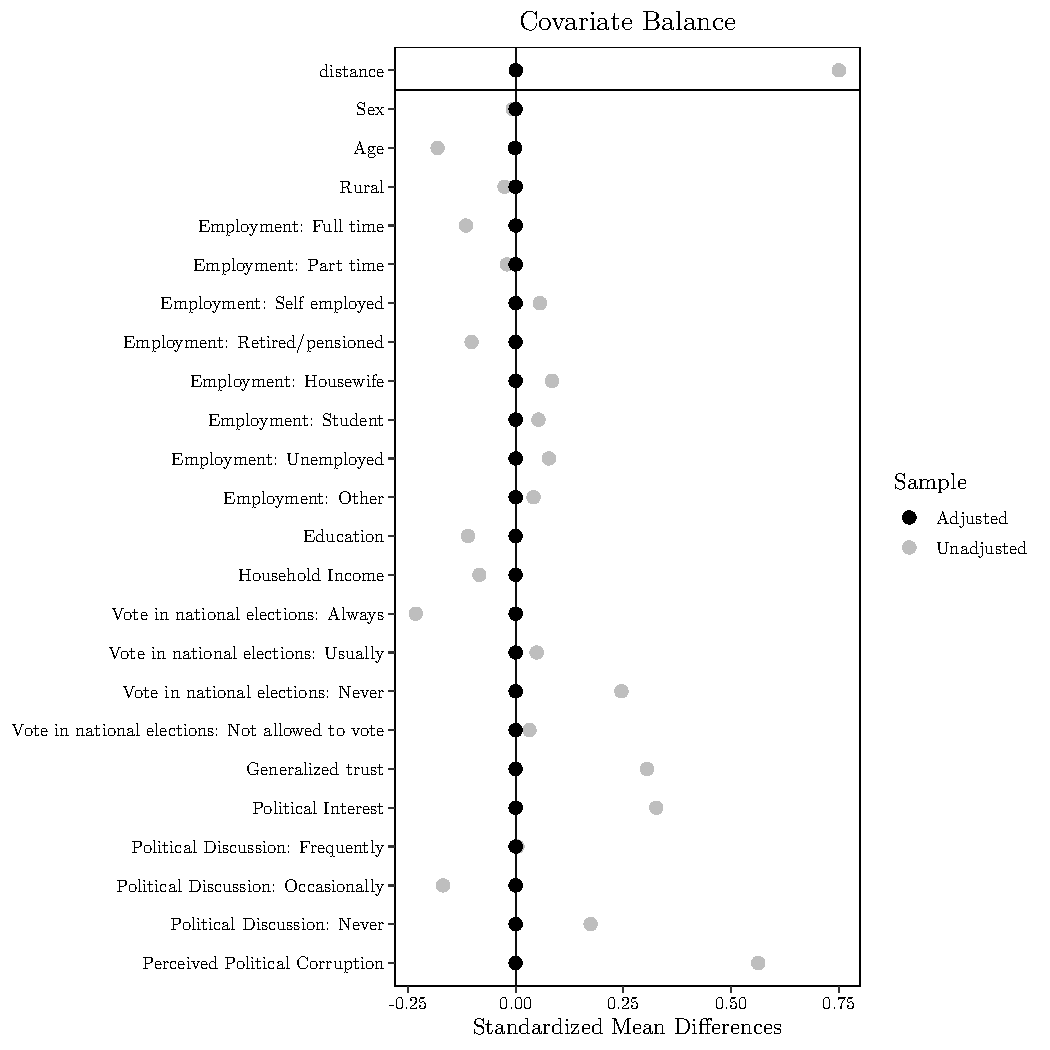
\includegraphics[width=0.9\linewidth]{covbalance_cem.pdf}
    \label{fig:balance}
\end{figure}

We apply matching as our main method for covariate adjustment in order to avoid parametric assumptions that stem from more conventional statistical models for cross-sectional data and present causal estimates on the relation between election fraud perceptions and diffuse political support. Statistical matching is commonly described as “the most developed [..] strategy for causal analysis in observational studies” (\citealt{Pearl2010}) and the literature on causal inference from cross-sectional data has produced a large range of algorithms and approaches to achieve balanced datasets that are free of usually embedded  parametric assumptions. 

We employ two different strategies for our inferences. First, we exploit propensity scores as the most popular similarity criterion and pre-select a subset of our data in which `treated’ and `control’ units most closely resemble each other in pre-treatment characteristics. The gold standard in constructing balanced data is exact matching, though usually disregarded because it produces a large share of cases that are left unmatched creating trouble for effect identification stemming from small sample sizes. In our particular case in which we exploit a dataset with over 48,000 data points, we can nevertheless rely on exact matches and construct a balanced dataset covering 580 individuals. Second, the use of propensity scores as a characteristic to match on has been criticized more generally (\citealt{King2019}). As a second approach to causal inference, we rely on coarsened exact matching (CEM) as developed by (\citealt{Iacus2012}) which has been proposed as an alternative to propensity score-based methods and has the potential to reduce large parts of model dependence, bias and variance that are left unaccounted by conventional matching algorithms. We compared these two approaches to a number of other algorithms for sample adjustment using matching and find these provide us with the best covariate balance by far. 

Figure 1 presents measures of covariate balance between those individuals falling into the `fraud’ and `no fraud’ perception condition before and after our sample adjustment. For each covariate that we match on, we report the standardized bias as measured by the difference in means between both groups of individuals scaled by the pooled standard deviation. Dots to the right (left) of the dashed vertical line are indicative of a higher incidence of respective characteristics among those individuals that perceive the elections of their country as unfair (fair). As indicated by the grey circles, fraud perceptions are most prevalent among those individuals that report to never turn out to vote, obtain low levels of interpersonal trust, and perceive political corruption at large scale in their country. 

\begin{table}[]
\caption{Matching Estimates: Effect of Fraud Perceptions on Confidence in Political Institutions.}
\singlespace
\begin{tabular}{llllccccc}
\hline
                              & \multicolumn{2}{c}{Na{\"i}ve Estimate}                                         & \multicolumn{1}{c}{}          & \multicolumn{2}{c}{Coarsened Exact Matching} &                      & \multicolumn{2}{c}{Exact Matching}          \\
                              & \multicolumn{1}{c}{\textit{Coef.}} & \multicolumn{1}{c}{\textit{Std.Err.}} & \multicolumn{1}{c}{\textit{}} & \textit{Coef.}        & \textit{Std.Err.}    & \textit{}            & \textit{Coef.}       & \textit{Std.Err.}    \\ \cline{2-3} \cline{5-6} \cline{8-9} 
\textit{Real Spillover}       &                                    &                                       &                               & \multicolumn{1}{l}{}  & \multicolumn{1}{l}{} & \multicolumn{1}{l}{} & \multicolumn{1}{l}{} & \multicolumn{1}{l}{} \\
Effect on: Armed Forces       & -0.432                             & 0.019                                 &                               & -0.508                & 0.073                &                      & -0.384               & 0.151                \\
Effect on: Police             & -0.526                             & 0.019                                 &                               & -0.671                & 0.074                &                      & -0.681               & 0.153                \\
Effect on: Press              & -0.428                             & 0.019                                 &                               & -0.366                & 0.074                &                      & -0.215               & 0.155                \\
Effect on: Courts             & -0.601                             & 0.019                                 &                               & -0.803                & 0.075                &                      & -0.718               & 0.153                \\
                              &                                    &                                       &                               &                       &                      &                      &                      &                      \\
\textit{Endogenous Spillover} &                                    &                                       &                               &                       &                      &                      &                      &                      \\
Effect on: Government         & -0.694                             & 0.020                                 &                               & -0.709                & 0.074                &                      & -0.739               & 0.153                \\
Effect on: Parliament         & -0.660                             & 0.020                                 &                               & -0.745                & 0.076                &                      & -0.514               & 0.155                \\
Effect on: Political Parties  & -0.560                             & 0.020                                 &                               & -0.535                & 0.076                &                      & -0.434               & 0.158                \\ \hline
Covariate Adjustment          & \multicolumn{2}{c}{$\surd$}                                                & \multicolumn{1}{c}{}          & \multicolumn{2}{c}{$\surd$}                  &                      & \multicolumn{2}{c}{$\surd$}                 \\
$N$                             & \multicolumn{2}{c}{48,953}                                                 & \multicolumn{1}{c}{}          & \multicolumn{2}{c}{2,475}                    &                      & \multicolumn{2}{c}{580}                     \\ \hline
\end{tabular}
\textit{Note: Na{\"i}ve estimates are drawn from ordinal logistic mixed models nesting 52,105 individuals in 48 countries fitted with maximum likelihood estimation. Matching results are drawn from exact and coarsened exact matching with postmatching regression adjustment through parametric ordinal logistic models. Coefficients represent average treatment effects (ATE).}
\end{table}

Notably, these differences are almost completely reduced after pruning the data as a result of our matching algorithms, as indicated by the black dots. Standardized bias is close to zero for all covariates in the adjusted sample, and matched groups are highly similar on any of their observed characteristics.\footnote{This picture equivalently holds for standardized bias reduction using propensity-score based exact matching.} Hence, in our analysis, the remaining differences on diffuse political support that are still observed between both groups on our fraud indicator can be plausibly attributed to differences in election day fraud perceptions. 

Table 2 presents the effect estimates. The first column presents na{\"i}ve estimates drawn from an ordinal logistic mixed model on the whole dataset using available covariates as control variables. Columns 2 and 3 present the results of our matching estimators. All coefficients provide estimates of the average treatment effect (ATE). Across specifications, we find robust support for our main hypothesis of attitudinal spillover. Perceived prevalence of election day ballot fraud in the federal elections of one’s country shows to robustly decrease confidence in political institutions that are unrelated to electoral administration. These effects hold for those institutions that are potentially thought to be related to electoral malpractice (endogenous spillover) as well as for those institutions that are exogenous to election day procedures (genuine spillover effect). 

\section*{Conclusion}

Acquiring credible information about electoral fraud can hold several attitudinal consequences for the relationship between citizens and their political system. The literature investigating the citizen-system nexus have focused on behavioral consequences of exposed cheating such as engaging in popular protests and violent uprisings (\citealt{Daxecker2012}). Regarding the electoral process itself, scholars have linked fraud information to negative evaluations of electoral quality (\citealt{Robertson2017}) and withdrawals of support from candidates that are allegedly involved in fraudulent practices (\citealt{Reuter2019}) and the regime that surged out of an allegedly fraudulent election (\citealt{Williamson2020}). The present article set out to theorize and explain the effects that acquiring credible information about electoral malpractice exerts on their confidence and diffuse support for the political system as a whole. 

In this article, we have provided first evidence that perceptions of election fraud lead to decays in levels of diffuse support for the political system as a whole among the citizenry. This spillover effect of election process-related perceptions to other components of the political system suggests that extrapolate process-related information even towards other institutions that are unrelated to electoral administration. Specifically, analyzing 48,953 respondents from Wave 7 (2017-2020) of the World Values Survey, respondents who perceive the election process of their country as less free and fair expressed lower levels of confidence in an array of political institutions even after rigorous covariate adjustment through statistical matching techniques. 

Second, we extended the focus of the simple citizen-system nexus and theorized about conditions that amplify or prevent such attitudinal spillover effects to occur. Specifically, we placed our theoretical scrutiny around the interventions of third-party stems actors and formulated two contrasting arguments on the moderating role of court convictions of alleged fraud perpetrators for the spillover effect of election fraud information. Last, we outlined the set up of a pre-registered online survey experiment to be conducted with respondents in Mexico and Russia which traces the causal mechanism behind the main spillover effect and its dependence on the occurrence of within-system interventions of courts as a consequence to exposed cheating. 

The theory and evidence presented in this article have a number of significant implications for developing democracies as well as contemporary authoritarianism. For instance, it has been shown that citizens who place higher levels of trust in their political system are more likely to turn out to vote (\citealt{WANG2016291}). Since active participation in institutionalized forms of democratic engagement is crucial for countries undergoing processes of democratic consolidation, our findings suggest that election fraud information can hinder the process of domestic democratization even in future electoral events that go beyond the impact on individual electoral contests. 

Second, our findings hold implications for the practice of election monitoring itself. Our article well aligns with a set of studies that have highlighted the cost among civil society when election observation missions expose cheating (\citealt{Daxecker2012}). Our preliminary findings suggest that when large-scale observation missions that are perceived and framed as credible players in the field claim election malpractice to be at place, such exposure may have detrimental effects that may hinder, rather than foster, the consolidation of a democratic society. This is especially relevant against the backdrop of widespread criticism that has been voiced against recent election observation missions proclaiming early conclusions about electoral malpractice that later do not uphold more intensive scrutiny (\citealt{Idrobo2020}). Our article suggests that the impact that such erroneous allegations about clean electoral process exerts on individuals should not be underestimated. 

\singlespace
\bibliographystyle{apsr} 
\bibliography{fraud_experiment}

\newpage

\section*{Appendix}

\subsection*{Cross-National Evidence: Descriptive Statistics}

\begin{table}[!htbp] \centering 
  \caption{Summary Statistics of Key Variables, World Values Survey Wave 7 (2017-2020).} 
  \label{} 
\begin{tabular}{@{\extracolsep{5pt}}lccccccc} 
\\[-1.8ex]\hline 
\hline \\[-1.8ex] 
Statistic & \multicolumn{1}{c}{N} & \multicolumn{1}{c}{Mean} & \multicolumn{1}{c}{St. Dev.} & \multicolumn{1}{c}{Min} & \multicolumn{1}{c}{Pctl(25)} & \multicolumn{1}{c}{Pctl(75)} & \multicolumn{1}{c}{Max} \\ 
\hline \\[-1.8ex] 
Confidence in Armed Forces & 48,953 & 2.876 & 0.951 & 1 & 2 & 4 & 4 \\ 
Confidence in the Press & 48,953 & 2.320 & 0.880 & 1 & 2 & 3 & 4 \\ 
Confidence in the Police & 48,953 & 2.619 & 0.959 & 1 & 2 & 3 & 4 \\ 
Confidence in Courts & 48,953 & 2.558 & 0.962 & 1 & 2 & 3 & 4 \\ 
Confidence in Government & 48,953 & 2.385 & 0.996 & 1 & 2 & 3 & 4 \\ 
Confidence in Parliament & 48,953 & 2.182 & 0.948 & 1 & 1 & 3 & 4 \\ 
Confidence in Parties & 48,953 & 2.017 & 0.895 & 1 & 1 & 3 & 4 \\ 
Fraud Perception & 48,953 & 0.364 & 0.481 & 0 & 0 & 1 & 1 \\ 
Political Interest & 48,953 & 2.682 & 0.963 & 1 & 2 & 3 & 4 \\ 
Generalized Trust & 48,953 & 1.818 & 0.386 & 1 & 2 & 2 & 2 \\ 
Voting in National Elections & 48,953 & 1.557 & 0.822 & 1 & 1 & 2 & 4 \\ 
Sex & 48,953 & 1.512 & 0.500 & 1 & 1 & 2 & 2 \\ 
Age & 48,953 & 42.313 & 16.020 & 16 & 29 & 54 & 103 \\ 
Education & 48,953 & 4.043 & 1.479 & 1 & 3 & 5 & 6 \\ 
Employment Status & 48,953 & 3.192 & 2.044 & 1 & 1 & 5 & 8 \\ 
Household Income & 48,953 & 4.782 & 2.101 & 1 & 3 & 6 & 10 \\ 
Rural & 48,953 & 1.355 & 0.479 & 1 & 1 & 2 & 2 \\ 
Political Discussion & 48,953 & 2.220 & 0.647 & 1 & 2 & 3 & 3 \\ 
Perceived Political Corruption & 48,953 & 7.813 & 2.428 & 1 & 6 & 10 & 10 \\ 
\hline \\[-1.8ex] 
\end{tabular} 
\end{table} 

\subsection*{Covariate Balance for Exact Matching}

\begin{figure}[H]
    \caption{Covariate Balance Before and After Sample Adjustment Using Exact Matching.}
    \centering
    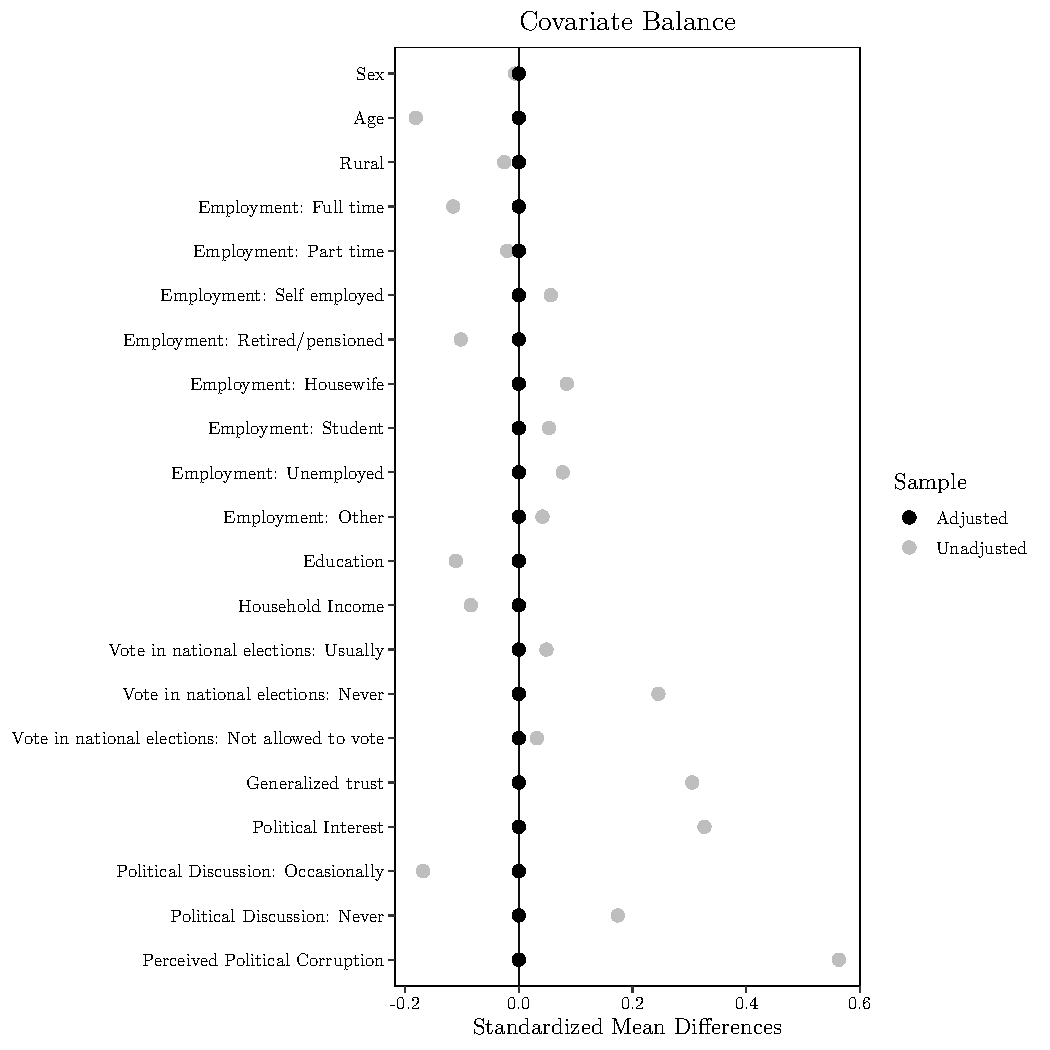
\includegraphics[width=0.9\linewidth]{covbalance_exact.pdf}
    \label{fig:balance}
\end{figure}

\newpage

\subsection*{Survey Experiment: Preliminary Questionnaire} 

\vspace{0.5cm}

\begin{center}
    POLITICAL ATTITUDES \\
\end{center}

\noindent \textbf{INT}. How much interest do you have in politics: A lot, some, little or none? \\
(1) A lot \\
(2) Some \\
(3) Little \\
(4) None \\

\noindent \textbf{PID1}. Do you currently identify with a political party? \\
(1) Yes \\
(2) No \\
(99) Don't know / Refusal \\

\noindent \textbf{PID2}. Which political party do you identify with? \\
\noindent [INSERT HERE] \\

\noindent \textbf{VOTE1}. Did you vote in the last presidential elections of [year of last presidential elections]? \\
(1) Voted \\
(2) Did not vote \\
(99) Don't know / Refusal \\

\noindent \textbf{VOTE2}. If there were a national legislative election tomorrow, for which party on this list would you vote? \\ \noindent [LIST OPTIONS HERE] \\

\noindent \textbf{LR}. Below you see portrayed a 1-10 scale that goes from left to right. The number one means left and 10 means right. Nowadays, when we speak of political leanings, we talk of those on the left and those on the right. In other words, some people sympathize more with the left and others with the right. According to the meaning that the terms "left" and "right" have for you, and thinking of your own
political leanings, where would you place yourself on this scale? \\

\noindent (1) \hspace{0.1cm} (2) \hspace{0.1cm} (3) \hspace{0.1cm} (4) \hspace{0.1cm} (5) \hspace{0.1cm} (6) \hspace{0.1cm} (7) \hspace{0.1cm} (8) \hspace{0.1cm} (9) \hspace{0.1cm} (10) \\
Left \hspace{6cm} Right \\

\noindent (99) Don't know / Refusal \\

\newpage

\noindent \textbf{CORRUP}. Now please let us know your views on corruption – when people pay a bribe, give a gift or do a favor to other people in order to get the things they need done or the services they need. How would you place your views on corruption in your country on a 10-point scale where “1” means “there is no corruption in my country” and “10” means “there is abundant corruption in my country”. If your views are somewhat mixed, choose the appropriate number in between. \\

\noindent (1) \hspace{0.1cm} (2) \hspace{0.1cm} (3) \hspace{0.1cm} (4) \hspace{0.1cm} (5) \hspace{0.1cm} (6) \hspace{0.1cm} (7) \hspace{0.1cm} (8) \hspace{0.1cm} (9) \hspace{0.1cm} (10) \\
No courruption \hspace{6cm} Abundant corruption \\

\noindent (99) Don't know / Refusal \\



\noindent \textbf{INTERT}. And speaking of the people from around here, would you say that people in this community are very trustworthy, somewhat trustworthy, not very trustworthy or
untrustworthy? \\
(1) Very trustworthy \\
(2) Somewhat trustworthy \\
(3) Not very trustworthy \\
(4) Untrustworthy \\
(99) Don't know / Refusal \\

\vspace{1cm}

\begin{center}
    TREATMENT AND OUTCOME
\end{center}

\noindent \textbf{SPLIT Control Group: Neutral Information} \\
On Sunday, \textit{[6 June 2021/19 September 2021]}, legislative elections are scheduled to be held in \textit{[Mexico/Russia]}. More than 2,000 registered candidates will compete for the \textit{[500/450]} parliamentary seats of the \textit{[Champer of Deputies/State Duma]}. The results will be determined by nearly \textit{[90/110]} million people in \textit{[Mexico/Russia]} and abroad. Suppose that as in the current convocation/parliament/as currently, four/seven parties retained positions. \\

%Suppose that federal legislative elections for the \textit{[Champer of Deputies/State Duma]} were held in \textit{[month]} of this year. Imagine that as usual, also in this hypothetical election more than 2,000 candidates competed for the \textit{[500/450]} parliamentary seats. Suppose that all parties that are currently presented in the \textit{[Champer of Deputies/State Duma]} have retained positions in the assembly and that the incumbent party \textit{[MORENA/United Russia]} has won the largest seat share. \\ as in the current convocation/parliament7as currently, four/seven parties retained positions. 

\noindent \textbf{SPLIT Treatment Group: Fraud Information} \\
\hl{$[$Neutral information$]$} \\
On an after election day, however, allegations of ballot-box stuffing and alterations of vote tallies perpetrated by individuals working for electoral commissions in favor of the incumbent party were widespread. Shortly after election day, a number of domestic and international election observation missions publicly called out a variety of electoral misconducts and manipulation practices across several regions of the country. \\

\noindent \textbf{SPLIT Treatment Group: Fraud Information With Electoral Commission Punishment} \\
\hl{$[$Neutral information$]$} \\
\hl{$[$Fraud information$]$} \\
As a consequence, individuals allegedly responsible for fraud lost their position in the electoral commissions that they served in. \\

\newpage

\noindent \textbf{SPLIT Treatment Group: Fraud Information With Court Punishment} \\
\hl{$[$Neutral information$]$} \\
\hl{$[$Fraud information$]$} \\
As a consequence, legal action was brought against individuals allegedly responsible for fraud which were convicted for electoral crimes by responsible courts. \\

\vspace{1cm}

\noindent Upon receiving this information, how much confidence would you have in the following organizations or institutions? Below you see a ladder with steps numbered 1 to 7, where 1 is the lowest step and means NOT AT ALL and 7 the highest and means A LOT. The ladder is followed by a series of questions. Please use the numbers provided in the ladder to answer. Remember, you can use any number. \\

\noindent (1) \hspace{1cm} (2) \hspace{1cm} (3) \hspace{1cm} (4) \hspace{1cm} (5) \hspace{1cm} (6) \hspace{1cm} (7) \\
Not at all \hspace{8cm} A lot \\

\noindent (99) Don't know / Refusal \\

\vspace{0.5cm}

\noindent \textbf{TRUST1}. To what extent do you trust the Armed Forces? \\

\noindent \textbf{TRUST2}. To what extent do you trust the Police? \\

\noindent \textbf{TRUST3}. To what extent do you trust the Press? \\

\noindent \textbf{TRUST4}. To what extent do you trust the Justice System/Courts? \\

\noindent \textbf{TRUST5}. To what extent do you trust the Government? \\
 
\noindent \textbf{TRUST6}. To what extent do you trust the Parliament? \\
 
\noindent \textbf{TRUST7}. To what extent do you trust the Political Parties? \\

\vspace{0.5cm}

\noindent \textbf{INVOLVE.} Some people say that there are systematic irregularities to be observed in the federal elections of [country], while other people deny that. Given that such claims were true, to which extent do you expect representatives of political parties and state-affiliated agents to be involved?”. \\
(1) Very involved \\
(2) Somewhat involved \\
(3) Not very involved \\
(4) Not at all involved \\
(99) Don't know / Refusal \\

\newpage

\begin{center}
    SOCIO-DEMOGRAPHICS \\
\end{center}

\noindent \textbf{SEX}. What sex are you? \\
(1) Female (2) Male (99) Don't know / Refusal \\

\noindent \textbf{URBAN}. Which size is the place you live at? \\
(1) National capital (metropolitan area) \\
(2) Large city ($>$ 500,000) \\
(3) Medium city ($>$ 100,000) \\
(4) Small city ($>$ 20,000) \\
(5) Rural area \\
(99) Don't know / Refusal \\

\noindent \textbf{BIRTH.} Can you tell me your year of birth, please? \\

\noindent \textbf{AGE}. This means you are ... years old. \textit{(write age in two digits)} \\

\noindent \textbf{IMMIG.} Were you born in this country or are you an immigrant to this country?  \\

\noindent \textbf{CITIZ.} Are you a citizen of this country? \\	

\noindent \textbf{EDU1}. What is the highest level of education you have attained? \\
(0) Early childhood education (ISCED 0) / no education  \\
(1) Primary education (ISCED 1) \\
(2) Lower secondary education (ISCED 2) \\
(3) Upper secondary education (ISCED 3) \\
(4) Post-secondary non-tertiary education (ISCED 4) \\
(5) Short-cycle tertiary education (ISCED 5) \\
(6) Bachelor or equivalent (ISCED 6) \\
(7) Master or equivalent (ISCED 7) \\
(8) Doctoral or equivalent (ISCED 8) \\
(99) Don't know / Refusal \\

\noindent \textbf{EDU2}. About how many years of education have you completed, whether full-time or part-time? Please report these in full-time equivalents and include compulsory years of schooling. \\
\noindent [INSERT HERE] \\

\noindent \textbf{OCCUP}. Which of these descriptions \underline{best} describes your current situation? \\
(1) In paid work (or away temporarily) (employee, self-employed, working for your family business) \\
(2) In education, (not paid for by employer) even if on vacation \\
(3) Unemployed and actively looking for a job 
(4) Unemployed, wanting a job but not actively looking for a job \\
(5) Permanently sick or disabled \\
(6) Retired \\
(7) In community or military service \\
(8) Doing housework, looking after children or other persons 
(9) Other \\
(99) Don't know / Refusal \\

\noindent \textbf{SECTOR}. Are you working for the government or public institution, for private business or industry, or for a private non-profit organization? If you do not work currently, characterize your major work in the past! Do you or did you work for: \\ 
(1) Government or public institution \\
(2)	Private business or industry \\
(3)	Private non-profit organization \\ 

\noindent \textbf{INC}. Which of the following descriptions comes closest to how you feel about your household’s income nowadays? \\
(1) Living comfortably on present income \\
(2) Coping on present income \\
(3) Finding it difficult on present income \\
(4) Finding it very difficult on present income \\
(99) Don't know / Refusal \\

\end{document}
